\documentclass{article}
\usepackage[T2A]{fontenc}
\usepackage[utf8]{inputenc}
\usepackage[russian,english]{babel}
\usepackage{graphicx}
\usepackage{float}
\graphicspath{ {./images/} }
 
\title{Определение систематических и случайных погрешностей при измерении удельного сопротивления нихромовой проволоки}
\author{Шахматов Андрей, Б02-304}
\date{\today}
  
\begin{document}

\maketitle

\begin{abstract}
    Измерено удельное сопротивление нихромовой проволоки различной длины.
    Для измерения сопротивления использовались два метода: анализ вольт-амперной характеристики, 
    полученной при помощи амперметра и вольтметра, и использование моста Уитстона с магазином сопротивлений. Получены значения удельных
    сопротивлений, измеренных двумя способами. Выявлено, что основной вклад в погрешность измерения удельного сопротивления проволоки 
    вносит погрешность измерения её диаметра, и потому нет различимой разницы в точности измерения двумя способами.
    Полученное значение удельного сопротивления оказалось в соответствии с табличными данными.
\end{abstract}

\tableofcontents

\section{Введение}

В современной электротехнике часто требуется проводить измерения удельных сопротивлений различных сплавов.
Один из самых распространённых методов - прямое измерение напряжения и тока на резисторе в участке цепи,
и дальнейшее получение сопротивления этого участка в результате анализа вольт-амперной характеристики. 
Такой метод не может обеспечить высокую точность измерений, 
так как результат может исказиться из-за наличия внутреннего сопротивления у вольтметра и амперметра.
Другим методом измерения сопротивления является использование моста Уитстона. Такой метод обеспечивает 
высокую точность, однако процесс измерения является трудноавтоматизируемым и дорогим, что делает его неподходящим для использования в промышленности.
Цель настоящей работы заключалась в расчёте систематических поправок при измерении сопротивления первым методом, используя второй 
метод в качестве эталонного, на примере измерения удельного сопротивления нихромовой проволоки. 

\section{Методика}
Для определения удельного сопротивления проволоки, считая проволоку однородной по длине, а её толщину - много меньше длины, 
можно применить следующее выражение:
\begin{equation}\label{eq:1}
    \rho = \frac{RS}{d}.
\end{equation}
Чтобы вычислить удельное сопротивление, следует найти длину $d$ и площадь сечения проволоки $S$.
Так как минимальная длина измеряемой проволоки - 0.3 м, для её измерения была выбрана линейка.
Толщина проволоки измерялась двумя инструментами: микрометром и штангенциркулем.
Для определения сопротивления были использованы амперметр и вольтметр. Характеристики проборов представлены в приложении~\ref{sec:app_1}
в таблице~\ref{tab:1}.

Для измерения сопротивления проволоки предполагалось использовать одну из двух схем, 
приведенных на рисунке~\ref{fig:1}.
\begin{figure}[H]
    \begin{center}
        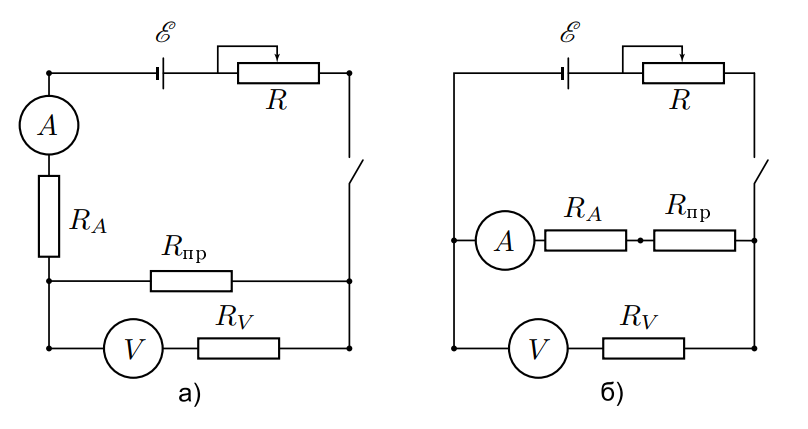
\includegraphics[width=\textwidth]{curcuits}
    \end{center}
    \caption{Схемы измерения сопротивления}
    \label{fig:1}
\end{figure}
С учётом предполагаемых значений сопротивления проволоки была выбрана первая схема (См. приложение \ref{sec:app_2}). \\
В качестве эталонного прибора для измерения сопротивления был использован мост Уитстона P4833.

\section{Результаты и их обсуждение}
\subsection{Измерение длины и площади сечения проволоки}
Сопротивление измерялось на трёх образцах проволоки различной длины: 20, 30 и 50 см.
Результаты измерений длины проволоки представлены в таблице \ref{tab:2}\\
Диаметр проволоки был измерен в 10 точках проволоки при помощи микрометра и штангенциркуля. 
Результаты измерения диаметра проволоки представлены в таблице \ref{tab:3}.
Получены следующие значения площади сечения и диаметра проволоки (См. приложение \ref{sec:app_4})
\begin{equation}
    d = (0.36 \pm 0.01) \textrm{ мм}
\end{equation}
\begin{equation}
    S = (0.101\pm0.006)\textrm{ мм}^2
\end{equation}
\subsection{Измерение сопротивления проволоки при помощи амперметра и вольтметра}
В таблицe~\ref{tab:4} указаны значения напряжения и силы тока, измеренные для использованных выше длин проволоки. 
Из графика~\ref{fig:2} следует, что значение удельного сопротивления не зависит от направления измерения, из чего следует, 
что для нихромовой проволоки результаты измерения тока не зависят от истории измерений.
\begin{figure}[H]
    \label{fig:2}
    \begin{center}
        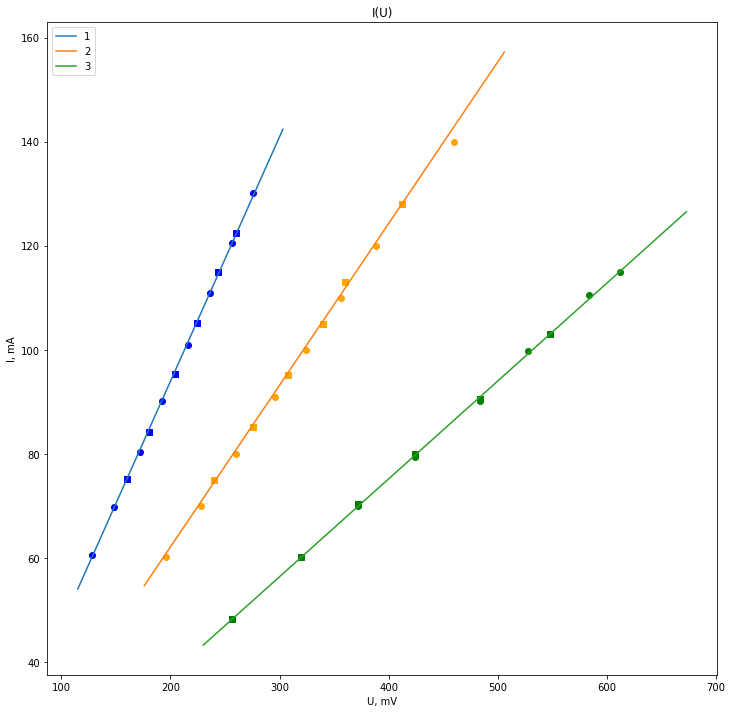
\includegraphics[width=\textwidth]{gr2} \\
    \end{center}
    \caption{Зависимость силы тока от напряжения, приложенного к нихромовой проволоке при различных её длинах: 
    1: l = 20 см, 2: l = 30 см, 3: l = 50 см.
    Кругами обозначены точки, полученные при увеличении значения напряжения, квадратами - полученные при уменьшении значения напряжения.
    Погрешности по оси I: $\sigma_I = 0.01 \textrm{ мА}$, по оси U: $\sigma_U = 2 \textrm{ мВ}$, что намного меньше масштабов графика, 
    потому кресты погрешностей не показаны.}
\end{figure}
Из графика следует, что полученная зависимость может быть апроксимированна прямой. Это означает, 
что для проволоки справедлив закон Ома и для неё можно ввести сопротивление $R$. 
Результаты вычисления коэффициентов наклона зависимостей, изображённых на рисунке~\ref{fig:2}, с помощью метода наименьших квадратов с нулевым
сдвигом по оси тока, представлены в таблицe~\ref{tab:5}. Вычисления представлены в приложении~\ref{sec:app_5}.
\begin{table}[H]
    \label{tab:5}
    \begin{center}
        \begin{tabular}{|r|r|r|r|}
            \hline
                           & l = 20 см & l = 30 см & l = 50 см \\
            \hline
            $R$, Ом        & 3.12      & 3.22      & 5.32      \\
            $\sigma_R$, Ом & 0.03      & 0.03      & 0.04      \\
            \hline
        \end{tabular}
    \end{center}
    \caption{Значения сопротивлений нихромовой проволоки при различных её длинах}
\end{table}
\subsection{Сравнение сопротивлений, полученных с использованием двух методов}
Сводные данные измерений двумя методами представлены в таблице \ref{tab:7}.
\begin{table}[H]
    \label{tab:7}
    \begin{center}
        \begin{tabular}{|l|r|r|r|}
            \hline
                                                     & l = 20 см           & l = 30 см           & l = 50 см           \\
            \hline
            $R_0, \textrm{ Ом}$                      & 2.1204 $\pm$ 0.0001 & 3.2227 $\pm$ 0.0001 & 5.3164 $\pm$ 0.0001 \\
            $R_{\textrm{ср}}, \textrm{ Ом}$          & 2.13 $\pm$ 0.04     & 3.22 $\pm$ 0.04     & 5.32 $\pm$ 0.05     \\
            $\sigma_R^{\textrm{случ}}, \textrm{ Ом}$ & 0.003               & 0.009               & 0.009               \\
            $\sigma_R^{\textrm{сист}}, \textrm{ Ом}$ & 0.04                & 0.04                & 0.05                \\
            \hline
        \end{tabular}
    \end{center}
    \caption{Сводная таблица измерений сопротивления нихромовой проволоки двумя способами:
    $R_0$ - сопротивление, измеренное с помощью моста Уитстона, $R_{\textrm{ср}}$ - сопротивление, измеренное при помощи амперметра и вольтметра. }
\end{table}
Из полученных данных можно сделать вывод, что значение сопротивления, измеренного при помощи амперметра и вольтметра, совпадает 
со значением, измеренным при помощи моста Уитстона. Основную долю погрешности измерения составляет приборная погрешность амперметра и вольтметра.
\subsection{Расчёт удельного сопротивления проволоки}
Результаты расчёта удельного сопротивления нихромовой проволоки и погрешность(приложение \ref{sec:app_6}) при различных её длинах 
представлены в таблице \ref{tab:8}.
\begin{table}[H]
    \label{tab:8}
    \begin{center}
        \begin{tabular}{|r|r|r|r|r|}
            \hline
            \multicolumn{3}{|c|}{Амперметр и вольтметр} & 
            \multicolumn{2}{|c|}{P4833}                                                                                                                                               \\
            \hline
            l, см                                       & p, $10^{-4}$ Ом$\cdot$см & $\sigma_p$, $10^{-4}$ Ом$\cdot$см & p, $10^{-4}$ Ом$\cdot$см & $\sigma_p$, $10^{-4}$ Ом$\cdot$см \\
            \hline
            20                                          & 1.08                     & 0.06                              & 1.07                     & 0.06                              \\
            30                                          & 1.09                     & 0.06                              & 1.09                     & 0.06                              \\
            50                                          & 1.08                     & 0.06                              & 1.08                     & 0.06                              \\
            \hline
        \end{tabular}
    \end{center}
    \caption{Удельное сопротивление нихромовой проволоки, полученное при различных длинах отрезков}
\end{table}

Значения удельного сопротивления оказались одинаковы в пределах погрешностей для обоих методов. Основной вклад в погрешность даёт слагаемое $(\frac{\sigma_S}{S})^2$
зависящее от погрешности измерения диаметра проволоки. Эта погрешность нивелирует различия в точности приборов, поэтому
можно считать, что для данной задачи не важен способ измерения сопротивления.
Среднее значение удельного сопротивления составило $\overline{\rho} = (1.08 \pm 0.04) 10^{-4}\textrm{ Ом}\cdot\textrm{см}$, что попадает в диапазон
$0.97\cdot10^{-4}\textrm{ Ом}\cdot\textrm{см}$ до $1.12\cdot10^{-4}\textrm{ Ом}\cdot\textrm{см}$ для сплавов нихрома при температуре
20 \textcelsius \cite{ValuesBook}.

\section{Выводы}
Значение удельного сопротивления нихромовой проволоки оказалось равно $(1.08 \pm 0.04) 10^{-4}\textrm{ Ом}\cdot\textrm{см}$ и совпало в пределах погрешности
с табличными данными. При этом полученные с помощью различных методов значения сопротивления нихромовой проволоки оказались одинаковы в пределах погрешности.
Источником погрешности удельного сопротивления является малая точность измерения диаметра проволоки.

\section{Использованная литература}
\begin{thebibliography}{9}
    \bibitem{LabBook}
    Лабораторный практикум по общей физике, Том 1, под редакцией А. Д. Гладуна
    
    \bibitem{ValuesBook}
    Физические величины. М. Энергоиздат, 1991. С. 444
    \end{thebibliography}

\section{Приложения}
\subsection{Характеристики измерительных приборов} \label{sec:app_1}
\begin{table}[H]
    \begin{tabular}{|l|l|l|}
        \hline
                                            & Вольтметр            & Миллиамперметр    \\
        \hline
        Система                             & Магнитоэлектрическая & Цифровая          \\
        Класс точности                      & 0.2                  & -                 \\
        Предел измерений $x_\textrm{п}$     & 0.6 В                & 2 А - 0.5 А       \\
        Число делений $x_\textrm{п}/n$      & 150                  & -                 \\
        Чувствительность $n/x_\textrm{п}$   & 4 мВ/дел             & -                 \\
        Абсолютная погрешность $\Delta x_M$ & 2 мВ                 & 0.006 мА - 0.6 мА \\
        Внутреннее сопротивление прибора    & 4000 Ом              & 1.2 Ом            \\
        \hline
    \end{tabular}
    \caption{Характеристики амперметра и вольтметра}
    \label{tab:1}
\end{table}
Погрешность штангенциркуля - 0.1 мм\\
Погрешность микрометра - 0.01 мм\\
Погрешность линейки - 0.5 мм.

\subsection{Расчёт поправок для сопротивления при измерении амперметром и вольтметром}\label{sec:app_2}

\begin{center}
    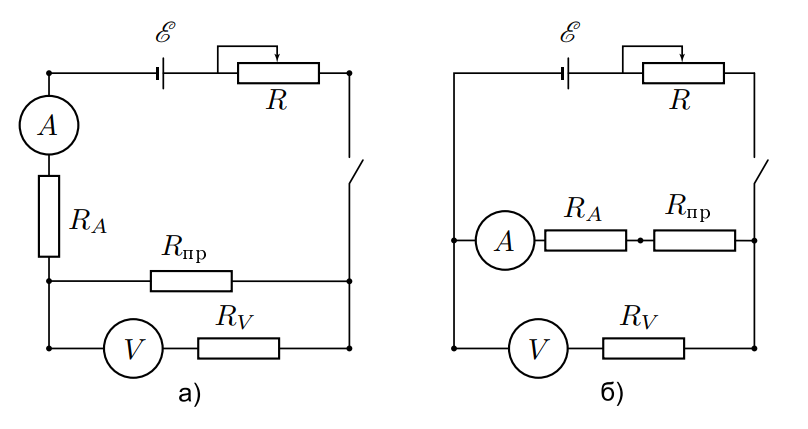
\includegraphics[width=\textwidth]{curcuits} \\
\end{center}
Для первой схемы:
$$R_{ \textrm{изм}} = R_{ \textrm{пр}}\frac{R_V}{R_{ \textrm{пр}} + R_V}$$
$$R_{ \textrm{пр}} = R_{ \textrm{изм}}\frac{R_V}{R_V - R_{ \textrm{изм}}} \approx R_{ \textrm{изм}}(1 + \frac{R_{ \textrm{изм}}}{R_V})$$
Для второй схемы:
$$R_{ \textrm{изм}} = R_{ \textrm{пр}} + R_A$$
$$R_{ \textrm{пр}} = R_{ \textrm{изм}}(1 - \frac{R_{ \textrm{изм}}}{R_A})$$
Где $R_{ \textrm{пр}}$ - реальное сопротивление проволоки\\
$R_{ \textrm{изм}}$ - измеренное сопротивление\\
$R_V$ - сопротивление вольтметра\\
$R_A$ - сопротивление амперметра.\\
Для измерения сопротивления проволоки, сопротивлением порядка 5 Ом, относительные поправки будут равны:
$$\epsilon_{R_a} = \frac{R}{R_v} \approx 0.1\%$$
$$\epsilon_{R_b} = \frac{R_a}{R} \approx 24\%$$

\subsection{Данные результатов измерений}\label{sec:app_3}
\begin{table}[H]
    \label{tab:2}
    \begin{center}
        \begin{tabular}{|l|l|l|l|}
            \hline
            $l$, см                  & 20 см  & 30 см  & 50 см  \\
            \hline
            $\sigma_l$, мм           & 0.5 мм & 0.5 мм & 0.5 мм \\
            \hline
            $\frac{\sigma_l}{l}, \%$ & 2.5    & 1.7    & 1.0    \\
            \hline
        \end{tabular}
    \end{center}
    \caption{Результаты измерения длины проволоки}
\end{table}
\begin{table}[H]
    \label{tab:3}
    \begin{center}
        \begin{tabular}{|l|l|l|l|l|l|l|l|l|l|l|}
            \hline
                      & 1    & 2    & 3    & 4    & 5    & 6    & 7    & 8    & 9    & 10   \\
            \hline
            $d_1$, мм & 0.4  & 0.4  & 0.4  & 0.4  & 0.4  & 0.4  & 0.4  & 0.4  & 0.4  & 0.4  \\
            $d_2$, мм & 0.36 & 0.35 & 0.36 & 0.35 & 0.36 & 0.36 & 0.36 & 0.36 & 0.36 & 0.37 \\
            \hline
        \end{tabular}
    \end{center}
    \caption{Результаты измерения диаметра проволоки, $d_1$ - измерения штангенциркулем, $d_2$ - измерения микрометром}
\end{table}
\begin{table}[H]
    \label{tab:4}
    \begin{tabular}{|c|r|r|r|r|r|r|r|r|r|r|r|}
        \hline
        \multicolumn{4}{|c|}{l = 20см} & 
        \multicolumn{3}{|c|}{l = 30см} & 
        \multicolumn{3}{|c|}{l = 50см}                                                                            \\
        \hline
                                       & V, дел & V, мВ & I, мА & V, дел & V, мВ & I, мА & V, дел & V, мВ & I, мА \\
        \hline
        0                              & 32     & 128   & 60.5  & 49     & 196   & 60.1  & 64     & 256   & 48.3  \\
        1                              & 37     & 148   & 69.8  & 57     & 228   & 70.0  & 80     & 320   & 60.2  \\
        2                              & 43     & 172   & 80.4  & 65     & 260   & 80.0  & 93     & 372   & 70.0  \\
        3                              & 48     & 192   & 90.1  & 74     & 296   & 90.9  & 106    & 424   & 79.5  \\
        4                              & 54     & 216   & 101.0 & 81     & 324   & 100.0 & 121    & 484   & 90.1  \\
        5                              & 59     & 236   & 111.0 & 89     & 356   & 110.0 & 132    & 528   & 99.8  \\
        6                              & 64     & 256   & 120.5 & 97     & 388   & 120.0 & 146    & 584   & 110.5 \\
        7                              & 69     & 276   & 130.1 & 115    & 460   & 140.0 & 153    & 612   & 115.0 \\
        0                              & 65     & 260   & 122.5 & 103    & 412   & 128.0 & 137    & 548   & 103.0 \\
        1                              & 61     & 244   & 115.0 & 90     & 360   & 113.0 & 121    & 484   & 90.5  \\
        2                              & 56     & 224   & 105.2 & 85     & 340   & 105.0 & 106    & 424   & 80.0  \\
        3                              & 51     & 204   & 95.3  & 77     & 308   & 95.2  & 93     & 372   & 70.3  \\
        4                              & 45     & 180   & 84.3  & 69     & 276   & 85.2  & 80     & 320   & 60.1  \\
        5                              & 40     & 160   & 75.2  & 60     & 240   & 75.0  & 64     & 256   & 48.3  \\
        \hline
    \end{tabular}
    \caption{Измерение напряжения и силы тока}
\end{table}
\begin{table}[H]
    \label{tab:6}
    \begin{center}
        \begin{tabular}{|l|l|l|l|}
            \hline
                                         & l = 20 см & l = 30 см & l = 50 см \\
            \hline
            $R_0, \textrm{ Ом}$          & 2.1204    & 3.2227    & 5.3164    \\
            $\sigma_{R_0}, \textrm{ Ом}$ & 0.0001    & 0.0001    & 0.0001    \\
            \hline
        \end{tabular}
    \end{center}
    \caption{Измерение сопротивления на приборе P4833}
\end{table}

\subsection{Анализ результатов измерения толщины проволоки и расчёт площади сечения} \label{sec:app_4}
При измерении штангенциркулем точность результата определяется только точностью прибора:
$$d_1 = (0.40 \pm 0.05) \textrm{ мм}$$
При измерении микрометром погрешность складывается из систематической($d_c$) и случайной($d_r$):
$$\sigma_{d_r}^2 = 0.01 \textrm{ мм}$$
$$\sigma_{d_c}^2 = \frac{1}{N}\sqrt{\sum_{i=1}^{n}{(d_i - \overline{d})}} \approx 2\cdot10^{-3} \textrm{ мм}$$
$$\sigma_{d_2} = \sqrt{\sigma_{d_r}^2 + \sigma_{d_c}^2} \approx 0.01 \textrm{ мм}$$
Так как $\sigma_{d_r}^2 >> \sigma_{d_c}^2$, можно считать проволоку однородной по диаметру, а значит выполняется формула \ref{eq:1}.
Получено, что погрешность диаметра проволоки, при измерении штангенциркулем, больше чем, погрешность при измерении
микрометром, потому в дальнейших вычислениях использованы значения диаметра, полученные при помощи микрометра.
Тогда введём площадь поперечного сечения проволоки:
$$S = \frac{\pi{d_2^2}}{4} \approx 0.101\textrm{ мм}^2$$
$$\sigma_S = 2S\frac{\sigma_d}{d} \approx 0.006\textrm{ мм}^2$$
$$S = (0.101\pm0.006)\textrm{ мм}^2$$

\subsection{Расчёт коэффициентов наклона и их погрешностей}\label{sec:app_5}
Формула для расчёта коэффициента и погрешности:
$$k = \frac{\overline{x}\overline{y}}{\overline{x^2}}$$
$$\sigma_k = \frac{1}{\sqrt{n}}\sqrt{\frac{\overline{y^2}}{\overline{x^2}} - k^2}$$
В этой формуле считается, что известно, что y(0) = 0.
\subsection{Расчёт удельных сопротивлений и погрешностей}\label{sec:app_6}
Формула для расчёта удельного сопротивления:
$$\rho = \frac{Rl}{S}$$
Формула погрешности:
$$\sigma_{\rho} = \rho\sqrt{(\frac{\sigma_R}{R})^2 + (\frac{\sigma_S}{S})^2 + (\frac{\sigma_l}{l})^2}$$


\end{document}